Dopo aver parlato di segnali a tempo continuo e segnali a tempo discreto, il nostro obbiettivo ora e' scrivere un algoritmo per modificare un segnale. In generale questa operazione sara' fatta costruendo dei filtri (o SISTEMI) che hanno in ingresso un segnale a tempo discreto ed in uscita sempre un segnale a tempo discreto.

\section{Esempio di sistemi, equazione alle differenze}
Troviamo un modo matematico per esprimere gli algoritmi.
Un operatore matematico che si applica ad un segnale tempo discreto e' detto \textbf{equazione alle differenze}, il quale ha in uscita un segnale tempo discreto ed in uscita sempre un segnale a tempo discreto.

Vediamo ora degli esempi di sistemi. Innanzitutto diamo delle definizioni, chiameremo n (la variabile indipendente) \textbf{presente}, di conseguenza considereremo un segnale con in input solo n, input presente.
Mentre considereremo un segnale $x[n - k], k \in \mathbf{N}$, \textbf{input passato}, invece un segnale $x[n + k], k \in \mathbf{N}$, \textbf{input futuro}. $y[n]$ e' considerato l'\textbf{output}

\[\begin{split}
    y[n] &= (x[n])^2 \\
    y[n] &= (x[n])^3 - x[n-1] + \frac{1}{2} x[n+1]
\end{split}\]

\section{Proprieta' dei sistemi}
\begin{itemize}
    \item Causale: sistema che dipende dal presente e dal passato: $y[n] = x[n-1]$
    \item Anti-Causale: sistema che dipende dal futuro $y[n] = x[n+2]$
    \item A-Causali: sistema che dipende sia dal passato che dal futuro: $y[n] = \frac{x[n+1] - x[n-1]}{2}$
\end{itemize}

\begin{figure}[ht!]
    \centering
    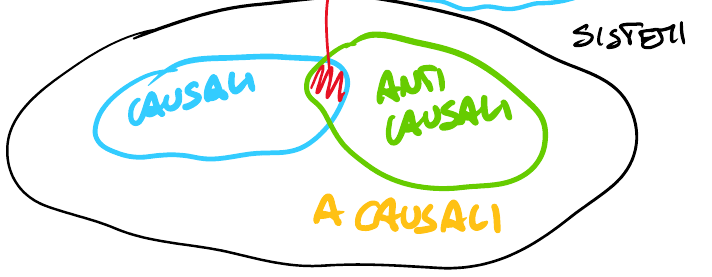
\includegraphics[scale=0.35]{immagini/lez12/sistemi.jpg}
\end{figure}

\section{Definizione di segnali tempo discreti particolari}
Diamo ora delle definizioni di segnali particolari che ci serviranno successivamente.

\subsection{Delta di Kronecker (impulso discreto)}
E' un segnale che vale 1 nel punto 0 e 0 in tutti gli altri punti. Ha quindi la caratteristica di essere estremamente collocato nel tempo.

\[\begin{split}
    \delta[n] = 
    \begin{cases}
    1 \text{ se } n = 0 \\
    0 \text{ se } n \ne 0 \\
    \end{cases}
\end{split}\]

Equivale alla modellazione discreta di un evento ad impulsi, ad esempio lo scoppio di un palloncino.

\begin{figure}[ht!]
    \centering
    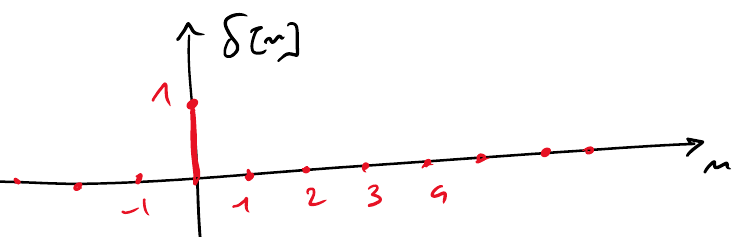
\includegraphics[scale=0.35]{immagini/lez12/delta.jpg}
\end{figure}

\subsection{Gradino causale (step function)}

\[\begin{split}
    u[n] = 
    \begin{cases}
    1 \text{ se } n \le 0 \\
    0 \text{ se } n < 0 \\
    \end{cases}
\end{split}\]

Possiamo considerarlo come un segnale che si attiva in un certo istante e poi rimane attivo all'infinito.

\begin{figure}[ht!]
    \centering
    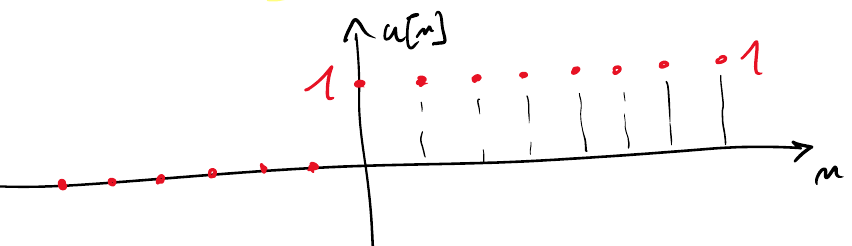
\includegraphics[scale=0.35]{immagini/lez12/gradinoCausale.jpg}
\end{figure}

\subsection{Gradino anticausale}
E' l'opposto del gradino causale:

\[\begin{split}
    -u[-n-1] = 
    \begin{cases}
    0 \text{ se } n \ge 0 \\
    -1 \text{ se } n < 0 (n \le 1) \\
    \end{cases}
\end{split}\]

Possiamo considerarlo come un segnale che esisteva da meno infinito in passato ed ad un certo punto finisce.

\begin{figure}[ht!]
    \centering
    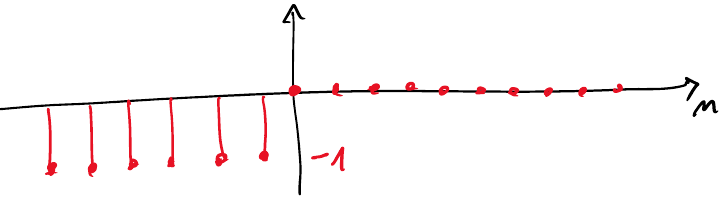
\includegraphics[scale=0.35]{immagini/lez12/gradinoAnticausale.jpg}
\end{figure}

\section{Altre poprieta' dei sistemi}

\subsection{Tempo-Invarianza (invarianza temporale)}

E' un concetto che possiamo facilmente ricondurre alla realta', noi ci aspettiamo sempre che se rifacciamo un'azione a distanza di tempo l'output derivato da quell'azione e' lo stesso, ad esempio riprodurre la stessa canzone una volta la mattina ed una la sera, ci aspettiamo che la canzone riprodotta sia la medesima.

Nell'esempio vediamo che se ritardiamo l'input di $n_0$ campioni, allora anche l'output e' ritardato degli stessi campioni $n_0$.

Vediamo ora degli esempi di tempo invarianza, vediamo come nel primo esempio, avendo un segnale tempo invariante (non dipendente da n), nonostante applichiamo un ritardo, all'ingresso o all'uscita del sistema, l'output non cambia. 
Mentre nel secondo caso il sistema $nx[n]$ e' strettamente dipendente ( dalla n che moltiplica il sistema) notiamo che gli outpu applicando il ritardo prima o dopo il sistema cambiano, quindi non e' tempo invariante. Generalizzando possiamo dire che un segnale che dipende strettamente dal tempo non e' a tempo invariante.

\begin{figure}[ht!]
    \centering
    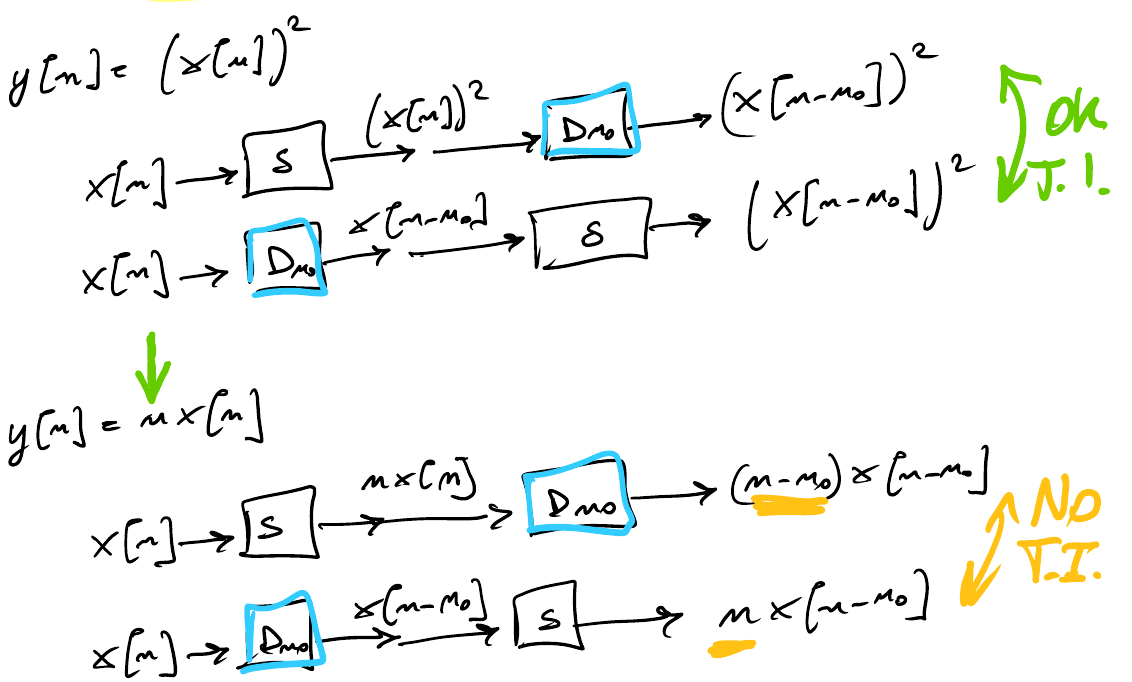
\includegraphics[scale=0.35]{immagini/lez12/esTempoInvarianza.jpg}
\end{figure}

Vedendolo in modo piu' "informatico" possiamo considerare il ritardo come se spostassimo di $n_0$ posizioni un array.

\begin{figure}[ht!]
    \centering
    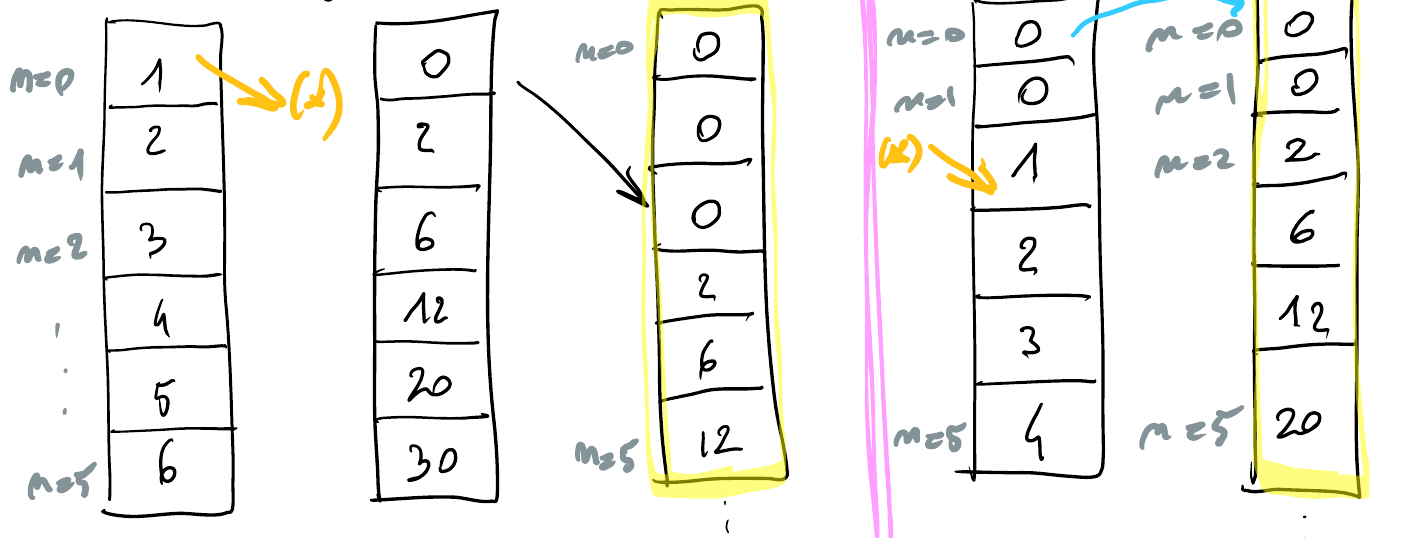
\includegraphics[scale=0.35]{immagini/lez12/tempoInvarianzaArray.jpg}
\end{figure}

\subsection{Linearita'}
Avendo un sistema con 2 input $x_1[n], x_2[n]$ e registro gli output del sistema $y_1[n], y_2[n]$, se invece mettiamo in input delle combinazioni lineari degli intput: $\alpha x_1[n], \beta x_2[n]$, ci sara' ancora una relazione con gli input precedenti?
Si se il sistema e' lineare, ed otterremo una combinazione lineare degli ouput di prima con gli stessi coeficienti degli input :$\alpha y_1[n], \beta y_2[n]$

\begin{figure}[ht!]
    \centering
    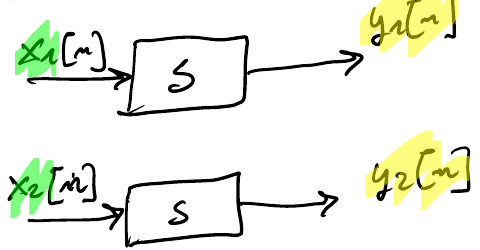
\includegraphics[scale=0.35]{immagini/lez12/linearita.jpg}
\end{figure}

Quello che facciamo in pratica e' dare degli stimoli al sistema e vederne gli effetti.

\section{Di che sistemi trattiamo}
In questo corso tratteremo solo di segnali lineare e tempo invarianti (LTI).

\begin{figure}[ht!]
    \centering
    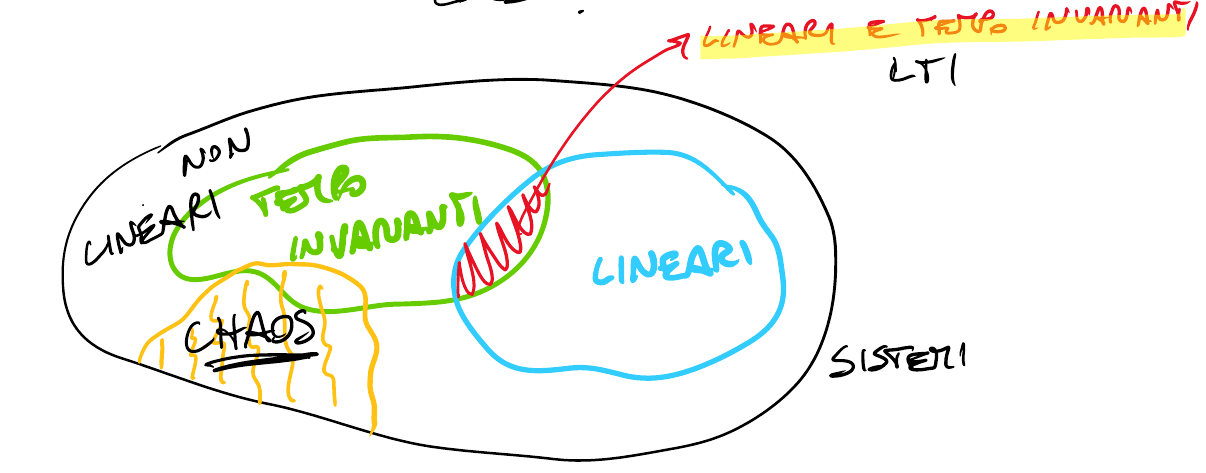
\includegraphics[scale=0.35]{immagini/lez12/sistemiTrattiamo.jpg}
\end{figure}

Notiamo che ci sono dei sistemi che godono della proprieta' del CHAOS, ovvero hanno estrema dipendente dalle condizioni iniziali.

\subsection{Esempio}
Prendiamo un input e lo mettiamo in un sistema.

In questo esempio useremo una delta nel sistema e notiamo che in uscita dal sistema abbiamo ancora una delta. Quello che facciamo quindi e' aver calcolato la \textbf{risposta del sistema} quando l'ingresso e' un impulso discreto, \textbf{risposta all'impulso}.

\[\begin{split}
    y[n] &= (x[n])^2 \\
    x[n] &= \delta[n] \\
    y[n] &= (\delta[n])^2 = \delta[n]
\end{split}\]

\begin{figure}[ht!]
    \centering
    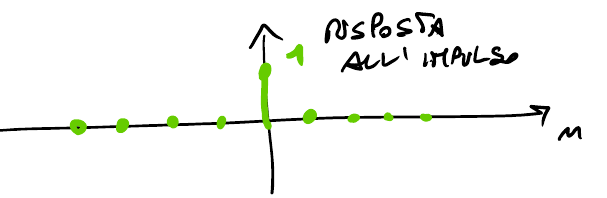
\includegraphics[scale=0.35]{immagini/lez12/esA.jpg}
\end{figure}

Ora cambiamo il sistema (sempre lineare e tempo invariante, LTI), e ci mettiamo sempre in input la delta e calcoliamo la risposta del sistema:

\[\begin{split}
    y[n] &= \frac{1}{2} x[n] + \frac{1}{2} x[n-1] \\
    x[n] &= \delta[n] \\
    y[n] &= h[n] = \frac{1}{2} \delta[n] + \frac{1}{2} \delta[n-1]
\end{split}\]

Per disegnare il grafico del segnale, notando che e' la somma di due funzioni delta, prendiamo la prima la dividiamo per 2, ovvero dove valeva 1 ora vale $\frac{1}{2}$ e dove valeva 0 rimane a 0, alla quale sommo un'altra funzione delta anch'essa divisa per 2 e traslata verso destra di 1 (perche' come sappiamo sottrarre un numero dalla variabile dipendente della funzione significa traslare verso destra la funzione del valore sottratto).

\begin{figure}[ht!]
    \centering
    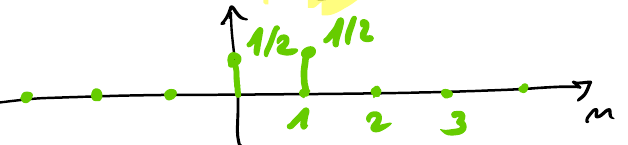
\includegraphics[scale=0.35]{immagini/lez12/esB.jpg}
\end{figure}

\section{Scomposizione con delta traslate}
Osserviamo che qualunque segnale puo' essere scomposto come somma di impulsi opportunamente scalati e traslati.

Disegniamo un segnale qualunque $x[n]$ che ha un supporto compatto, ovvero ha un dominio limitato nel tempo (e' definito nel tempo in un certo intervallo). Notiamo che ogni campione del segnale puo' essere scritto come una funzione delta scalata di un valore (l'altezza y) e traslata sull'asse x.

\begin{figure}[ht!]
    \centering
    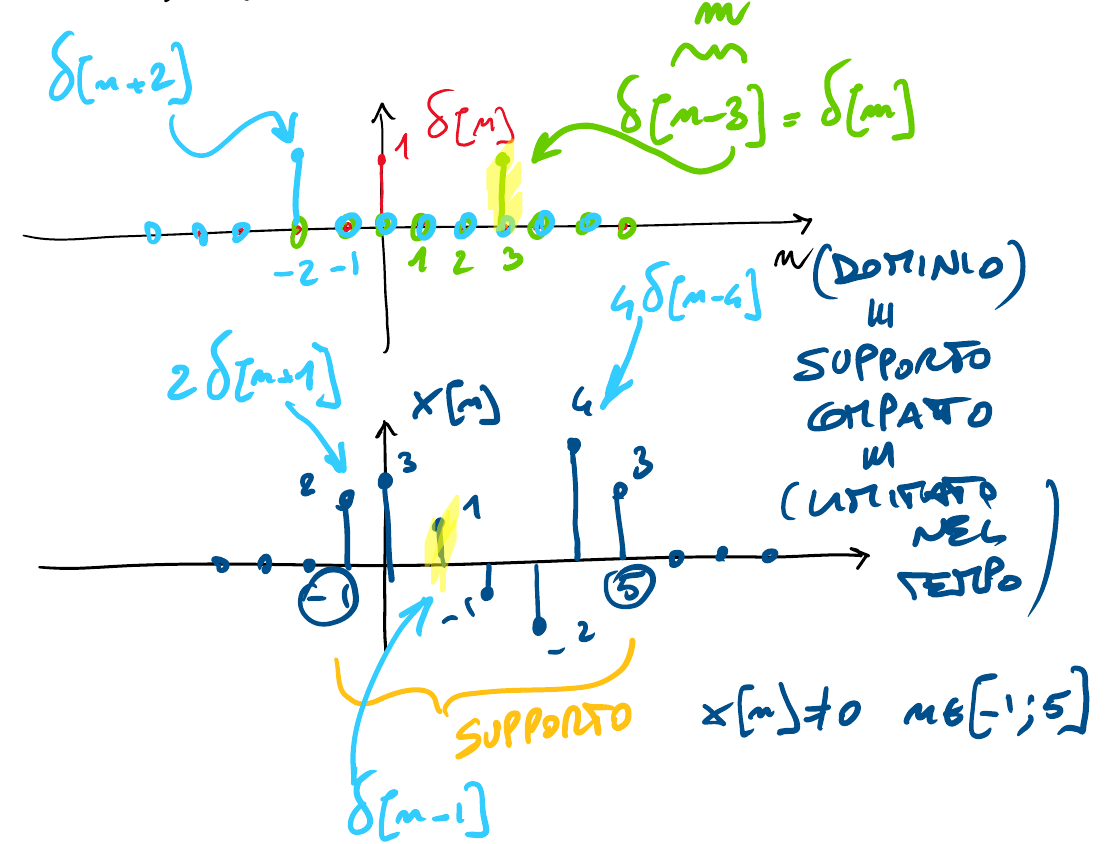
\includegraphics[scale=0.35]{immagini/lez13/composizioneDelta.jpg}
\end{figure}

Riscriviamo quindi il segnale come composizione di delta:
\[
    x[n] = 2 \delta[n+1] + 3 \delta[n] + \delta[n-1] - \delta[n-2] -2 \delta[n-3] + 4 \delta[n-4] + 3 \delta[n-5]
\]

Questa cosa possiamo farla con qualsiasi segnale:

\[
    x[n] = \sum_{k = - \infty}^{+\infty} x[k] \delta[n-k]
\]

dove $x[n]$ e' il valore del segnale nel punto (la modulazione delle y), $\delta[n-k$ e' la funzione delta traslata nel tempo. Inoltre notiamo che generalizzando si puo' scomporre un segnale anche che non abbia un supporto compatto.

Ci serve per descrivere in modo naturale un segnale, un insieme di campioni nel tempo con valori diversi.

\section{Prodotto di convoluzione}
Vediamo che la risposta all'impulso (che esiste sempre) per i sistemi lineari e tempo invarianti ci permette di descrivere le uscite dal sistema per qualunque segnale.

Consideriamo quindi un sistema generale, con input $x[n]$ ed output $y[n]$. Possiamo scrivere $y[n]$ come composizione lineare degli $x[n]$, inoltre posso anche sostituire al segnale $x[n]$ la sommatoria di funzione delta (come abbiamo appena visto), ottenendo:

\[
    y[n] = L(\sum_{k = - \infty}^{+ \infty} x[k] \delta[n-k])
\]

quindi possiamo usare la linearita' dell'operatore lineare L, dato che $x[n]$ e' un numero:

\[
    y[n] =\sum_{k = - \infty}^{+ \infty} x[k] L(\delta[n-k])
\]

il nostro sistema e' anche tempo invariante, abbiamo spostato l'input ($\delta[n-k]$), quindi mi aspetto che anche l'output sia spostato nel tempo ($h[n-k]$).

\begin{figure}[ht!]
    \centering
    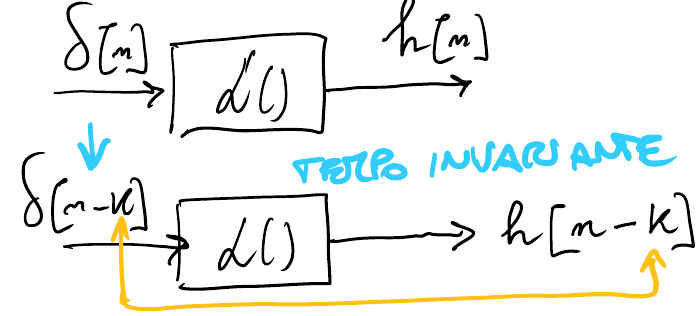
\includegraphics[scale=0.35]{immagini/lez13/tempoInvarianteConvoluzione.jpg}
\end{figure}

\[
    y[n] =\sum_{k = - \infty}^{+ \infty} x[k] h[n-k]
\]

Quindi se conosciamo $h[n]$ possiamo calcolare $y[n]$ qualsiasi sia l'input. La risposta all'inpulso caratterizza perfettamente il mio sistema.
L'operazione si chiama prodotto di convoluzione:

\[
    \sum_{k = - \infty}^{+ \infty} x[k] h[n-k] = x[n] * h[n]
\]

\subsection{Proprieta' del prodotto di convoluzione}

\subsubsection{Commutativa}
\[\begin{split}
    y[n] &= x[n] * h[n] = \sum_{k = - \infty}^{+ \infty} x[k] h[n-k] \\
    y[n] &= h[n] * x[n] = \sum_{k = - \infty}^{+ \infty} h[k] x[n-k]
\end{split}\]

\subsubsection{Associativa}
\[\begin{split}
    (x[n] * y[n]) * z[n] = x[n] * (y[n] * z[n])
\end{split}\]

\subsubsection{Distributiva rispetto alla somma}
\[\begin{split}
    (x[n] + y[n]) * z[n] = x[n] * z[n] + y[n] * z[n]
\end{split}\]

\subsubsection{Elemento neutro}
\[\begin{split}
    x[n] * e[n] &= x[n] \\
    e[n] &= \delta[n] \\
    x[n] * \delta[n] &= \sum_{k = - \infty}^{+ \infty} x[k] \delta[n-k] = x[n]
\end{split}\]

\subsection{Razionalizzando la convoluzione}

Riscriviamo la convoluzione ribaltando e la traslazione nel tempo:

\[
    \sum_{k = - \infty}^{+ \infty} x[k] h[n-k] = h[-(k-n)]
\]

\section{Risposta in frequenza}

\begin{figure}[ht!]
    \centering
    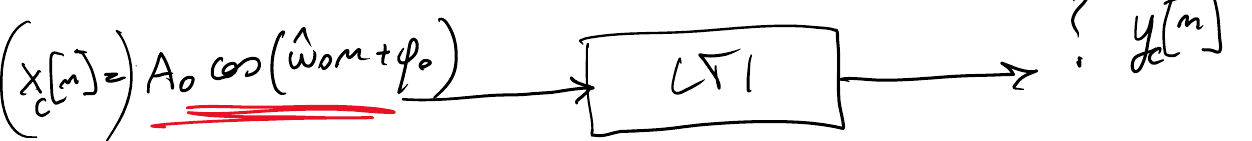
\includegraphics[scale=0.35]{immagini/lez13/cosinusoideDiscreta.jpg}
\end{figure}

Possiamo scomporre con Eulero la cosinusoide:

\[\begin{split}
    \sum_{k = -\infty}^{+\infty} \frac{A_0}{2} \{ e^{\hat{\omega_0} k i} e^{i \varphi_0} + e^{- \hat{\omega_0} k i} e^{- i \varphi_0} \} h[n-k]\\
    \mbox{Separiamo la sommatoria sulla somma} \\
    \sum_{k = -\infty}^{+\infty} \frac{A_0}{2} \{ e^{\hat{\omega_0} k i} e^{i \varphi_0} h[n-k] \} + &\sum_{k = -\infty}^{+\infty} \frac{A_0}{2} \{ e^{- \hat{\omega_0} k i} e^{- i \varphi_0} h[n-k] \} \\
    \mbox{Portiamo fuori i termini costanti che non dipendono da k} \\
    \frac{A_0}{2} e^{i \varphi_0} \cdot \sum_{k = -\infty}^{k = +\infty} e^{+i \hat{\omega_0}k} h[n-k] + \frac{A_0}{2} e^{-i \varphi_0} \cdot \sum_{k = -\infty}^{k = +\infty} e^{-i \hat{\omega_0}k} h[n-k] \\
    \mbox{Notiamo che ci sono termini che sono complessi e complessi coniugati} \\
    \mbox{Applichiamo ora la proprieta' commutativa della convoluzione} \\
    \frac{A_0}{2} e^{i \varphi_0} \cdot \sum_{k = -\infty}^{k = +\infty} e^{+i \hat{\omega_0}(n-k)} h[k] + \frac{A_0}{2} e^{-i \varphi_0} \cdot \sum_{k = -\infty}^{k = +\infty} e^{-i \hat{\omega_0}(n-k)} h[k] \\
    \mbox{Posso applicare le proprieta' delle potenze} \\
    e^{\hat{\omega_0}(n-k)i} = e^{\hat{\omega_0} n i} e^{-\hat{\omega_0} k i} \\
    \mbox{Porto fuori i termini che non dipendono da k} \\
    \frac{A_0}{2} e^{i \varphi_0} e^{\hat{\omega_0}n i} \cdot \sum_{k = -\infty}^{k = +\infty} e^{-\hat{\omega_0}k i} h[k] + \frac{A_0}{2} e^{-i \varphi_0} e^{-\hat{\omega_0} n i} \cdot \sum_{k = -\infty}^{k = +\infty} e^{\hat{\omega_0} k i} h[k] \\
\end{split}\]

Arrivati a questo punto notiamo che $\sum_{k = -\infty}^{k = +\infty} e^{-\hat{\omega_0}k i} h[k]$ e' un numero complesso ed e' importante, quindi lo chiamiamo $H(e^{j \hat{\omega_0}})$ che dipende da $\hat{\omega_0}$, l'altro e' il complesso coniugato: $H^*(e^{j \hat{\omega_0}})$.

L'output di un sistema $y[n]$ quando abbiamo in input una cosinusoide discreta:

\[
y[n] = H(e^{j \hat{\omega_0}}) \frac{A_0}{2} e^{i \varphi_0} e^{\hat{\omega_0}n i} + H^*(e^{j \hat{\omega_0}}) \frac{A_0}{2} e^{-i \varphi_0} e^{-\hat{\omega_0} n i}
\]

Ora riscriviamo i termini in H in forma polare (ricordando che la parte tra il modulo e' il modulo e l'esponenziale moltiplicato per il modulo e' la fase):

\[\begin{split}
    y_c[n] &= | H(e^{j \hat{\omega_0}}) | e^{i \varphi H(e^{j \hat{\omega_0}})} \cdot \frac{A_0}{2} e^{i \varphi_0} e^{\hat{\omega_0}n i} + | H(e^{j \hat{\omega_0}}) | e^{-i \varphi H(e^{j \hat{\omega_0}})} \cdot \frac{A_0}{2} e^{-i \varphi_0} e^{-\hat{\omega_0}n i} \\
    &\mbox{Raccolgo i termini con la stessa base} \\
    &= | H(e^{j \hat{\omega_0}}) | \frac{A_0}{2} e^{i[\hat{\omega_0} n + \varepsilon_0 + \varphi H (e^{j \hat{\omega_0}})]} + | H(e^{j \hat{\omega_0}}) | \frac{A_0}{2} e^{-i[\hat{\omega_0} n + \varepsilon_0 + \varphi H (e^{j \hat{\omega_0}})]} \\
    y_c[n] &= | H(e^{j \hat{\omega_0}} | A_0 \cos [ \hat{\omega_0} n + \varepsilon_0 + \varphi_0 H (e^{j \hat{\omega_0}})]
\end{split}\]

Concludendo notiamo che in output dal sistema abbiamo un coseno con la stesse frequenza discreta di qu
ello messo in input.
Si dice quindi che il coseno e' un autofunzione di un sistema LTI, ovvero che non viene modificata nella sua forma funzionale (ha la stessa frequenza), ma al massimo iene traslato in ampiezza e fase.

$H(e^{i \hat{\omega_0}})$ e' detta \textbf{risposta in frequenza del sistema} $\in \mathbf{C}$.

\[
    H(e^{i \hat{\omega_0}}) = \sum_{k = -\infty}^{+\infty} h[n] e^{-i \hat{\omega_0} k }
\]

Approfondiamo ora le proprieta' della risposta in frequenza.

\subsection{Chiarimento}
Notiamo che abbiamo scritto la risposta in frequenza come una funzione $H(e^{j \hat{\omega}})$ che quindi non dipende da una singola variabile ma da un esponenziale, questo perche':

\[
  H(e^{j \hat{\omega}}) = \sum_{n = - \infty}^{+\infty} h[n] e^{-j \hat{\omega} n} =  \sum_{n = - \infty}^{+\infty} h[n] e^{(j \hat{\omega})-n} 
\]

Notiamo quindi che e' una funzione del termine $e^{i \hat{\omega}}$.
Inoltre specifichiamo utilizzando Eulero $e^{i \hat{\omega}} = \cos \hat{\omega} + i \sin \hat{\omega}$, dato che compare nella risposta in frequenza anche quest'ultima e' quindi una funzione periodica di periodo $2\pi$.

\subsection{Simmetria coniugata}
Perche' abbiamo sia la risposta in frequenza sia la sua coniugata.
\[\begin{split}
    H(e^{j \hat{\omega}}) &= \{ H(e^{-j \hat{\omega}}) \}^* \\
    H(e^{j \hat{\omega}}) &= \sum_{n = - \infty}^{+ \infty} h[n] e^{-i \hat{\omega}n} \\
    H(e^{-j \hat{\omega}}) &= \sum_{n = - \infty}^{+ \infty} h[n] e^{-i (\hat{- \omega}) n} = \sum_{n = - \infty}^{+ \infty} h[n] e^{i \hat{\omega}n} \\
    (\sum_{n = - \infty}^{+ \infty} h[n] e^{i \hat{\omega}n})^* &= H(e^{j \hat{\omega}})
\end{split}\]

Quindi possiamo dire che la risposta in frequenza ha una parte reale che e' il mudolo che ha simmetria pari, ed una parte immaginaria che e' la fase con simmetria dispari.

\section{Supporto risposta all'impulso}
La risposta all'impulso si divide in due categorie:
\begin{itemize}
    \item FIR (Finite Impulse Response): se ho un supporto compatto allora si chiama risposta all'impulso finita, nel supporto e non nell'ampiezza (che e' finita di perse'). $h[n] \neq 0 \rightarrow n \in [a,b]$.
    \item IIR (Infinite Impulse Response): se non ha un supporto compatto si chiama risposta all'impulso infinita. $h[n] \neq 0 \rightarrow n < > a$
\end{itemize}

Abbiamo quindi una prima intuizione di filtro, in quanto la risposta all'impulso e' un filtro con cui calcoliamo l'uscita di un sistema.

\section{Equazione alle differenze di un qualunque sistema LTI}
Possiamo definire un'equazione alle differenze standard per qualunque sistema LTI:

\[
    y[n] = \sum_{h = -N_1, h \neq 0}^{N_2} a h y[n-h] + \sum_{k = -M_1}^{M_2} bk x[n-k]
\]

In cui $ah$ e $bk$ sono costanti, $y[n-h$ e' l'uscita del sistema futura o passata e $x[n-k]$ e' l'input del sistema (presente, passato o futuro).
La prima sommatoria si chiama parte \underline{AUTOREGRESSIVA (AR)} che dipende dall'output del sistema.
La seconda sommatoria si chiama \underline{MEDIA MOBILE (MA)} o MOUVING AVERAGE, che dipende solamente dall'input al sistema.
Se riusciamo a ricondurre l'equazione alle differenze di un sistema a questa equazione generale non dobbiamo verificarne la linearita' e la tempo invarianza.

Inoltre possiamo dire che condizione sufficiente (ma non necessaria) per un sistema LTI per avere risposta all'impulso finita (FIR) e' che $ah = 0, \forall h$. Vuol dire che non c'e' dipendenza dall'output ma solamente dall'input, ovvero non esiste la parte autoregressiva.

Notiamo inoltre che se e' presente la parte autoregressiva NON posso dire che il sistema non e' FIR.

\section{Filtraggio (pratico) con sistemi LTI}
Proviamo a capire perche' ci interessa la risposta all'impulso di un sistema.

\begin{figure}[ht!]
    \centering
    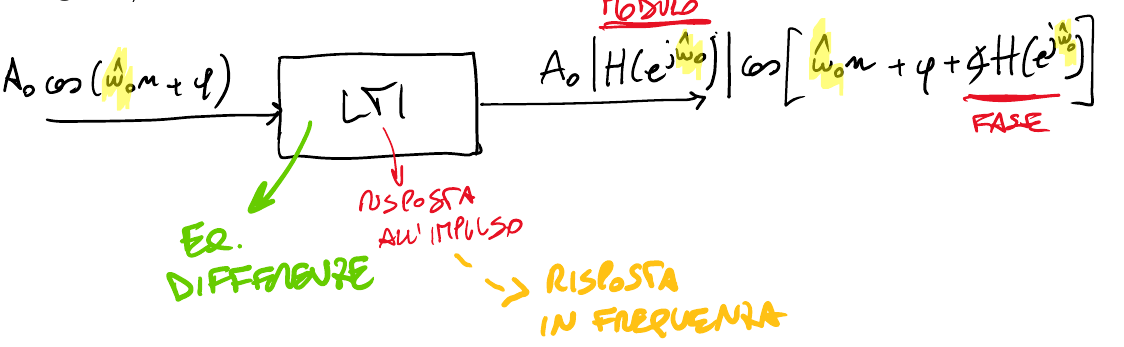
\includegraphics[scale=0.35]{immagini/lez15/uscitaLTIcoseno.jpg}
\end{figure}

Ricordiamo innanzitutto che l'uscita di sistema LTI quando l'input e' una cosinusoide discreta e' una cosinusoide discreta con la stessa frequenza ma modulata in modulo e fase.
Questa nozione e' alla base del filtraggio pratico con sistemi LTI.
Partiamo dall'ipotesi che abbiamo un segnale discreto da filtrare, che e' una combinazione lineare di cosinusoidi discrete. Quello che voglio fare e' fare agire il filtro tipo un setaccio, per far passare solo le cosinuosidi che mi interessano e scartare quelle che non mi interessano.
Notiamo che e' il modulo della risposta in frequenza che puo' fare questa operazione, in quanto se lo mettiamo uguale a 0 il coseno non esiste, quindi e' come se lo avessimo "bloccato".
Inoltre potremmo anche amplificare (o diminuire) l'ampiezza di una cosinusoide, se il modulo della risposta in frequenza fosse $\neq 0$.

Quindi il modulo della risposta in frequenza puo' aumentare o diminuire l'ampiezza (in verticale $\hat{|}$) della cosinusoide, mentre la fase ci permette di spostarla (in orizzontale $\leftrightarrow$) rispetto a quella che mettiamo in ingresso al sistema LTI.

\begin{figure}[ht!]
    \centering
    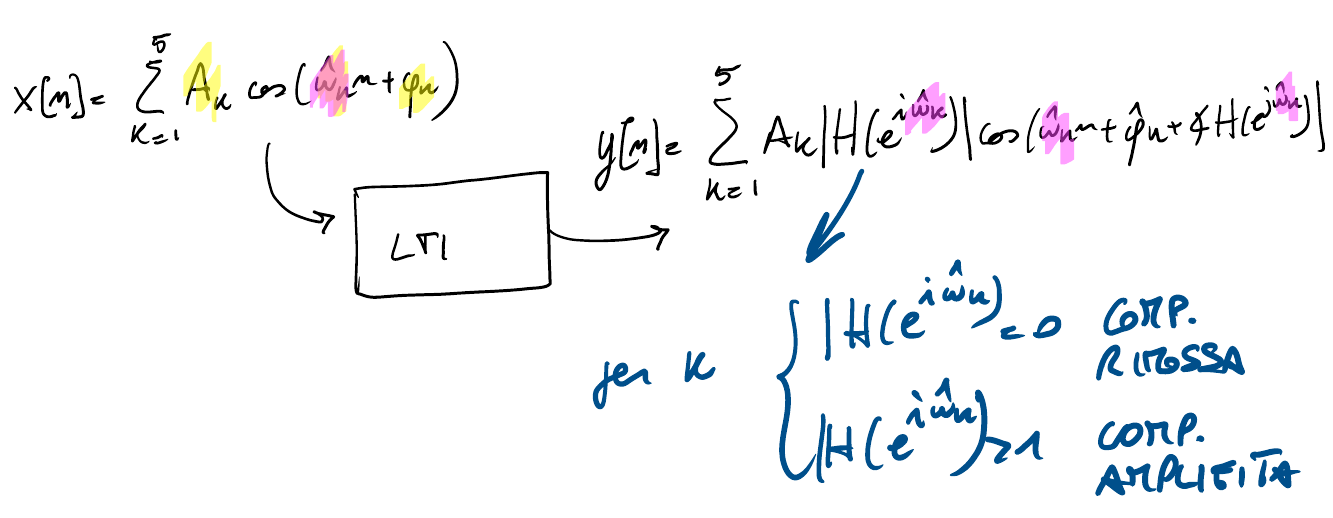
\includegraphics[scale=0.35]{immagini/lez15/filtraggioLTI.jpg}
\end{figure}

Sono stati definiti dei filtri ideali.

\subsection{Filtro passa basso (low pass)}
\begin{figure}[ht!]
    \centering
    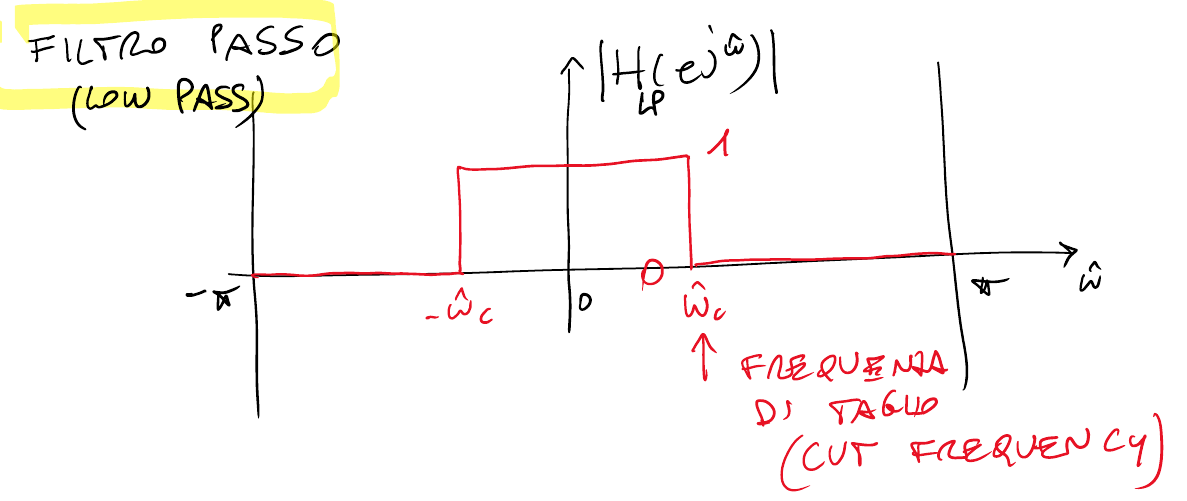
\includegraphics[scale=0.35]{immagini/lez15/passaBasso.jpg}
\end{figure}

Innanzitutto notiamo che il grafico del filtro e' rappresentato tra $-\pi, \pi$ questo perche' la risposta in frequenza e' periodica, quindi ci aspettiamo che fuori da questo intervallo si ripete.

Questo filtro ci dice che se consideriamo una frequenza (di una cosinuoside) compresa tra $-\hat{\omega}, \hat{\omega}$, dato che il filtro vale 1, la cosinuoside esce uguale a come e' entrata (in ampiezza), mentre tutte le cosinusoidi con frequenze fuori da questo intervallo vengono cancellate, perche' uscirebbero con ampiezza 0, in quanto il modulo della risposta in frequenza fuori dall'intervallo vale 0.

\subsection{Filtro passa alto (High Pass)}
E' il duale del filtro passa basso, quindi elimina tutte le cosinusoidi con frequenza compresa tra $-\hat{\omega}, \hat{\omega}$ e mantiene inalterate le altre.

\begin{figure}[ht!]
    \centering
    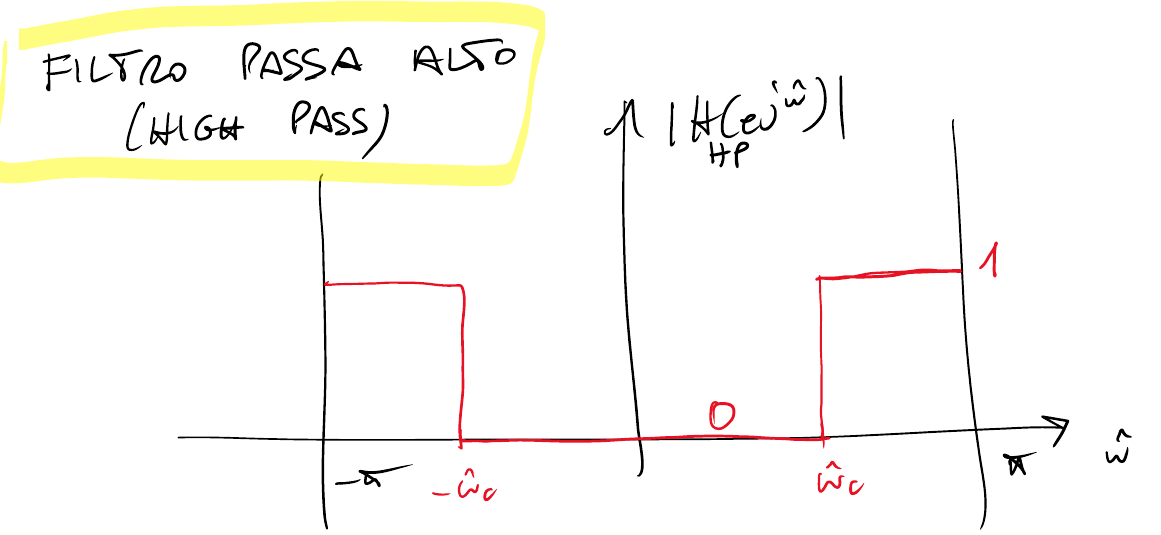
\includegraphics[scale=0.35]{immagini/lez15/passaAlto.jpg}
\end{figure}

Notiamo che se la frequenza di taglio del filtro passa alto e del passa basso e' uguale, allora dato un filtro posso riscrivere l'altro:

\[\begin{split}
    |H_{LP}(e^{j \hat{\omega}})| &= 1 - |H_{HP}(e^{j \hat{\omega}})| \\
    |H_{HP}(e^{j \hat{\omega}})| &= 1 - |H_{LP}(e^{j \hat{\omega}})| 
\end{split}\]

Dove $H_LP$ e' la risposta in frequenza del filtro passa basso e $H_HP$ e' la risposta in frequenza del filtro passa alto.

\subsection{Filtro passa banda (Band Pass)}
A volte serve uccidere frequenze alte e basse ma lasciare una certa banda.

\begin{figure}[ht!]
    \centering
    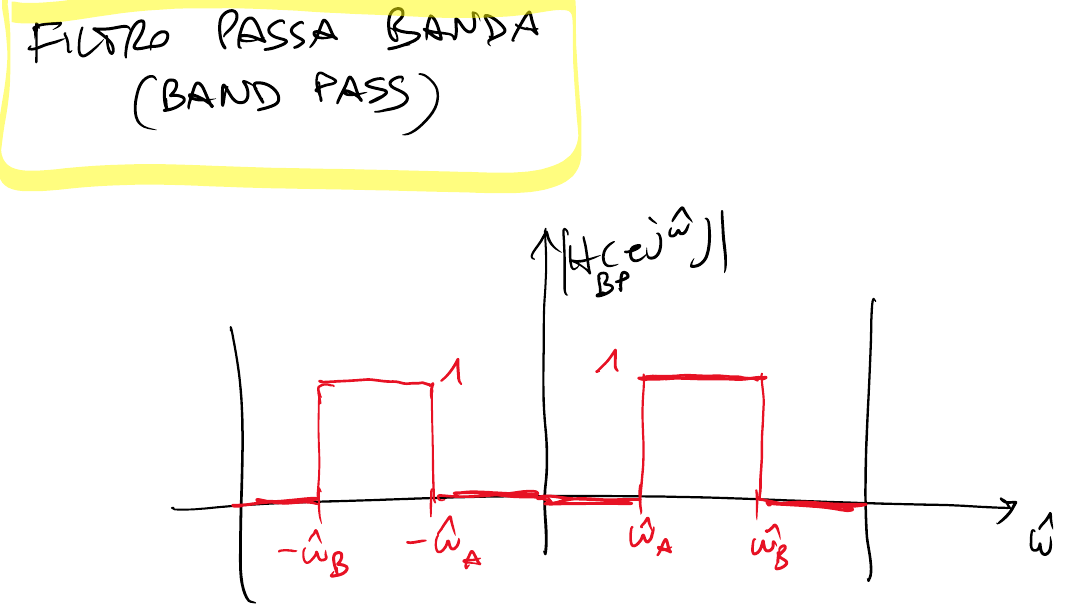
\includegraphics[scale=0.35]{immagini/lez15/passaBanda.jpg}
\end{figure}

\subsection{Filtro blocca banda (Band Block)}
E' il duale del filtro passa banda. Cancella le frequenze che appartengono ad una certa banda. Ad esempio e' usato quando vogliamo cancellare l'interferenza della rete elettrica, (50Hz), nel segnale campionato cancelleremo quel piccolo range di frequenze.

Si chiama Notch Filter quando la banda bloccata e' poco ampia.

\begin{figure}[ht!]
    \centering
    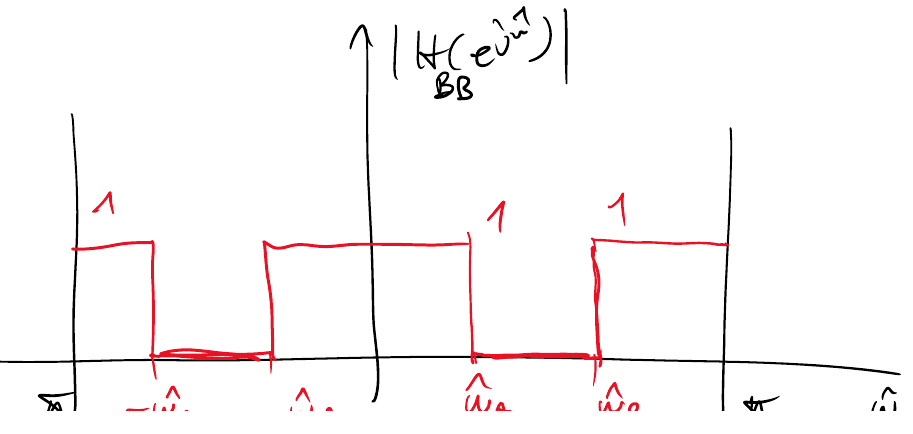
\includegraphics[scale=0.35]{immagini/lez15/bloccaBanda.jpg}
\end{figure}

Anche in questo caso, se la banda e' uguale, posso dato un filtro passa banda posso ottenere il blocca banda e viceversa:

\[
    |H_{BP}(e^{i \hat{\omega}})| = 1 - |H_{BB}(e^{i \hat{\omega}})|
\]



Queste sono definizioni di riferimento, ora vediamo degli esercizi in cui partendo da un equazione alle differenze scriviamo la risposta in frequenza e ne disegniamo il modulo e fase. Infine vedremo a quale filtro ideale assomiglia.

\subsection{Esercizio 1}

Abbiamo un filtro: $y[n] = x[n] + 2x[n-1] + x[n-2]$, quindi quando entra un input in questo sistema ne consideriamo 3 campioni, un presente e due passati, di conseguenza e' un sistema CAUSALE (in quanto dipende solo da presente e passato) e FIR in quanto non e' presente la parte autoregressiva (quella che dipende dall'output). Quindi posso scrivere la risposta all'impulso semplicemente sostituendo $x = \delta$:

\[
    h[n] = 1 \delta[n] + 2 \delta [n-1] + \delta[n-2]
\]

Ora dobbiamo calcolare la risposta in frequenza, per farlo notiamo che dalla sommatoria dobbiamo tenere solo gli elementi in cui la delta e' diversa da 0 (dove vale 1) e sono quelli che annullano la n dentro le varie delta. Mentre come coeficienti moltiplicativi usiamo quelli delle delta:

\[
    H(e^{i \hat{\omega}}) = \sum_{n = +\infty}^{-\infty} x[n] e^{-j \hat{\omega} n} = 1 e^{-j \hat{\omega} 0} + 2 e^{-j \hat{\omega} 1} + 1 e^{-j \hat{\omega} 2}
\]

Ora per trovare il modulo e la fase dobbiamo fare qualche operazione algebrica:

\[
    1 + 2 e^{-j \hat{\omega}} + 1 e^{-j \hat{\omega} 2}
\]

ora il consiglio per risolvere questa equazione e' raccogliere la meta' del termine massimo e vedere cosa succede:

\[
    2e^{-j \hat{\omega}} \{ \frac{e^j \hat{\omega}}{2} + 1 + \frac{e^{-j \hat{\omega}}}{2} \}
\]

Usando Eulero noto che $\frac{e^j \hat{\omega}}{2} + \frac{e^{-j \hat{\omega}}}{2} = \cos(\hat{\omega})$, quindi:

\[
    2e^{-j \hat{\omega}} [1 + \cos(\hat{\omega})]
\]

Ora invece di trasformare in forma polare riscrivo l'equazione in modo che sia scritta in maniera simile alla forma polare, che ricordiamo essere $\phi e^{i \Omega}$, da cui posso ricavare il modulo e la fase:

\[
    (2 + 2 \cos(\hat{\omega}) e^{-j \hat{\omega}}
\]

Dato che $2 + 2 \cos(\hat{\omega} \ge 0$ e' il modulo e la fase sara' $-\hat{\omega}$.

\begin{figure}[ht!]
    \centering
    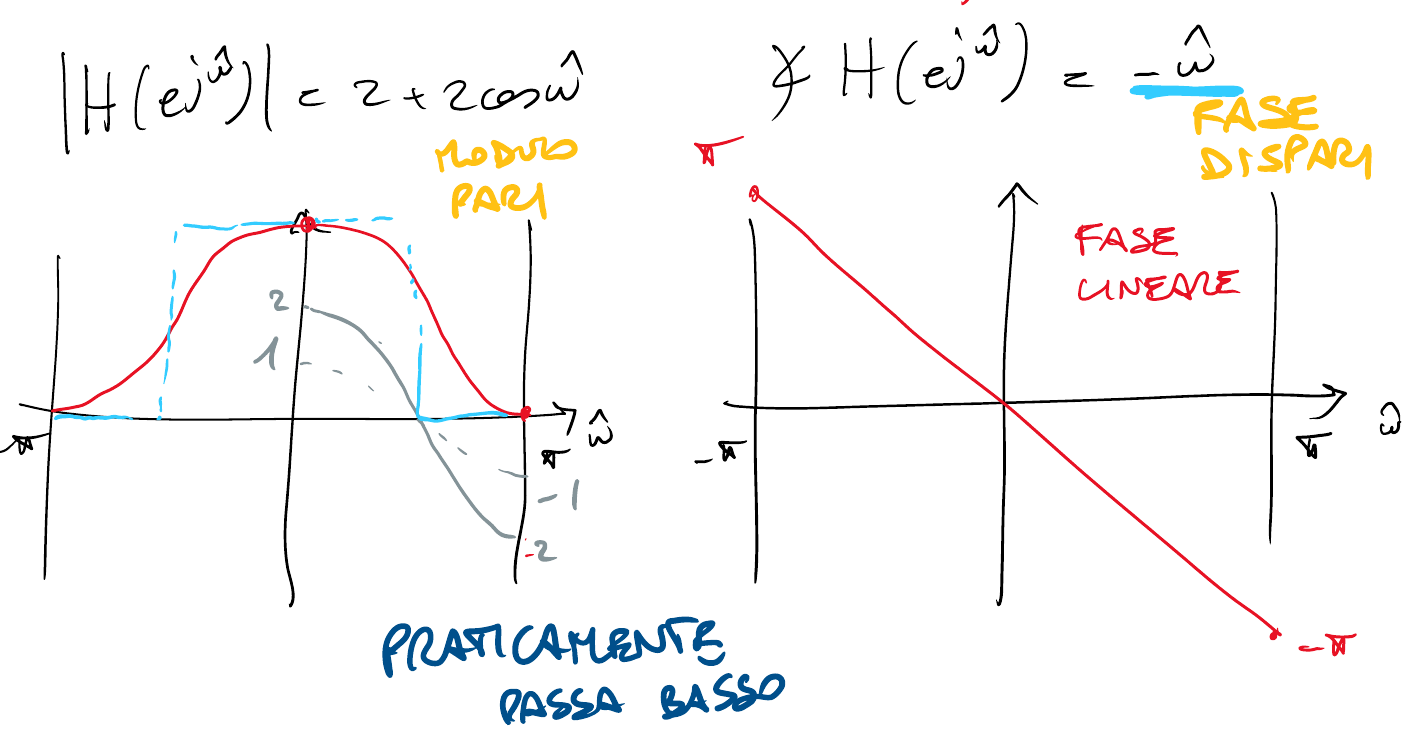
\includegraphics[scale=0.35]{immagini/lez15/es1.jpg}
\end{figure}

Per disegnare i grafici semplicemente dobbiamo disegnare il grafico di ciascuna funzione (modulo e fase), sempre nel periodo della risposta in frequenza $-\pi, +\pi$.
In questo caso notiamo dal grafico del modulo che questo e' un'approssimazione del filtro passa basso.

\subsection{Esercizio 2}
Usiamo lo stesso filtro di prima ma cambiando un segno $y[n] = x[n] - 2x[n-1] + x[n-2]$.
Seguiamo i passaggi fatti in precedenza, quindi inizialmente scriviamo la risposta all'impulso:
\[
    h[n] = 1 \delta[n] - 2 \delta [n-1] + \delta[n-2]
\]

Poi calcoliamo la risposta in frequenza:

\[
    H(e^{i \hat{\omega}}) = \sum_{n = +\infty}^{-\infty} x[n] e^{-j \hat{\omega} n} = 1 e^{-j \hat{\omega} 0} -
    2 e^{-j \hat{\omega} 1} + 1 e^{-j \hat{\omega} 2}
\]

\[\begin{split}
    H(e^{i \hat{\omega}}) &= 1 - 2 e^{-j \hat{\omega}} + 1 e^{-j \hat{\omega} 2} \\
    &= 2e^{-j \hat{\omega}} \{ \frac{e^j \hat{\omega}}{2} - 1 + \frac{e^{-j \hat{\omega}}}{2} \} \\
    &= 2e^{-j \hat{\omega}} [-1 + \cos(\hat{\omega})] \\
\end{split}\]

Ma arrivati a questo punto notiamo che $\cos(\hat{\omega}) - 1$ non puo' essere il modulo, in quanto non e' maggiore di 0. Notiamo che se togliamo un - sarebbe sempre positivo e quindi il modulo:
\[
    -1 e^{-j \hat{\omega}} (2 + 2 \cos(\hat{\omega}))
\]

Ma quel segno meno, come abbiamo sempre fatto, possiamo riscriverlo come $-1 = e^{j\pi}$.

\begin{figure}[ht!]
    \centering
    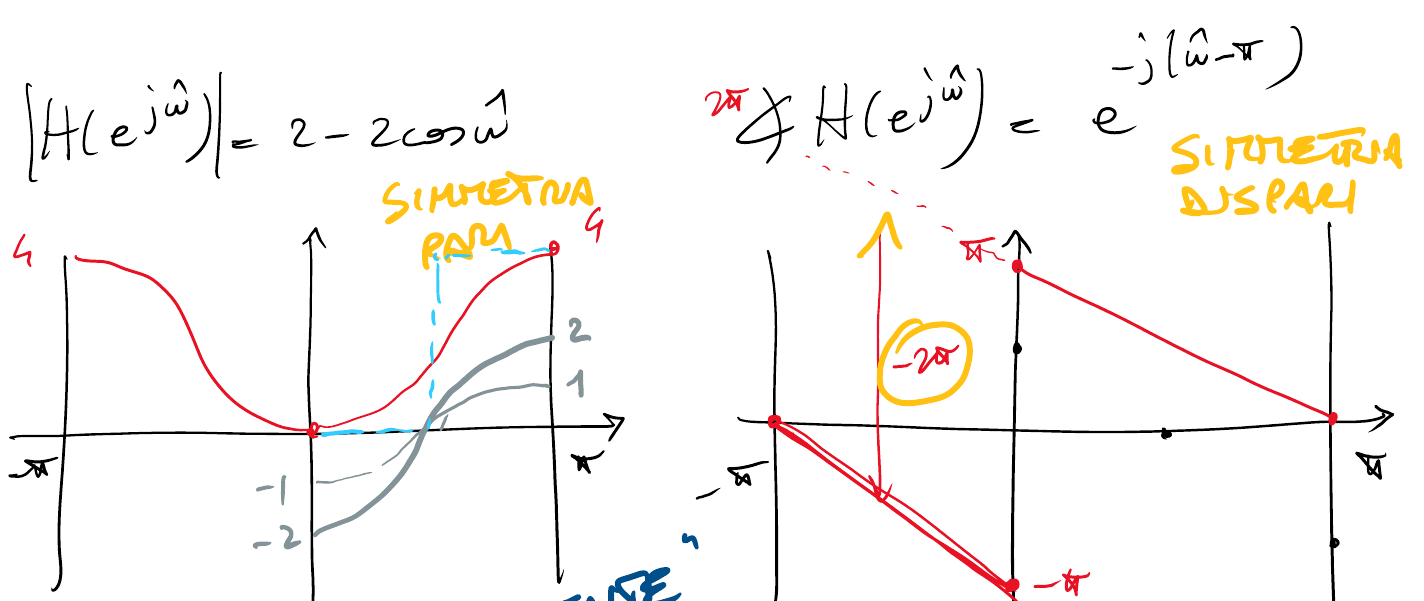
\includegraphics[scale=0.35]{immagini/lez15/es2.jpg}
\end{figure}

Dal grafico del modulo notiamo che e' un'approssimazione del filtro passa alto.

\subsection{Esercizio 3 (Amplificatore Ideale)}
Abbiamo un filtro $y[n] = Ax[n-n_0]$, in cui $n_0$ e' costante ed $A>0$. 
Notiamo subito che se $n_0 \ge 0$ il sistema e' CAUSALE e FIR.
Quello che fa in pratica questo filtro e' prendere il segnale e ritardarlo di n campioni e lo moltiplica di un valore A. Si chiama amplificatore ideale.
Come fatto in precedenza calcoliamo la risposta all'impulso:

\[
    h[n] = A \delta[n-n_0]
\]

Tracciamone il grafico:

\begin{figure}[ht!]
    \centering
    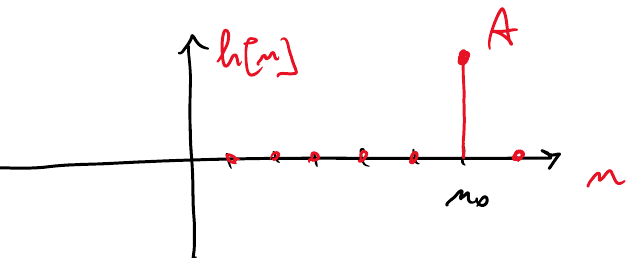
\includegraphics[scale=0.35]{immagini/lez15/es2RispostaImpulso.jpg}
\end{figure}

Troviamo la risposta in frequenza, come prima prendendo dalla sommatoria solo il termine in cui la delta vale 1, in questo caso l'argomento della delta si annulla quando $n = n_0$:

\[
    H(e^{i \hat{\omega}}) = A e^{-j \hat{\omega} n_0}
\]

Da cui ricaviamo il modulo $A$ e la fase $-\hat{\omega}n_0$.





\begin{figure}[ht!]
    \centering
    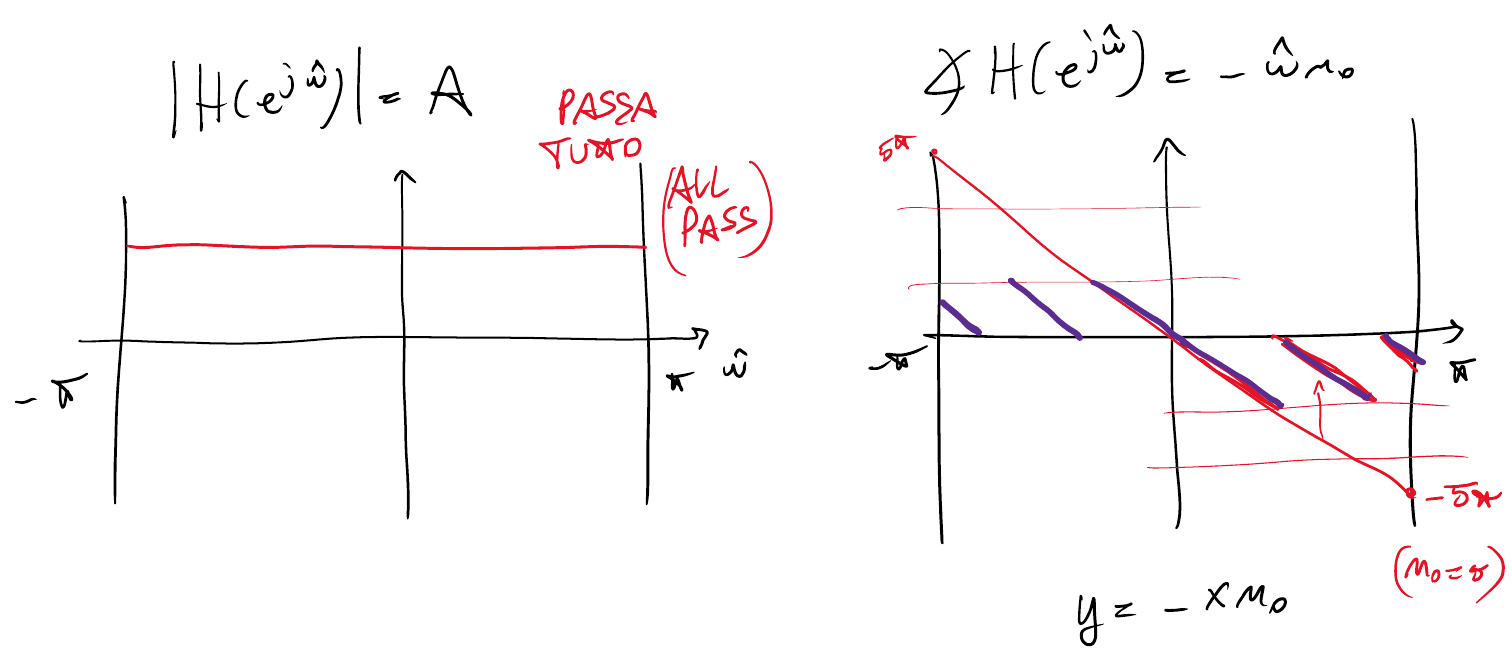
\includegraphics[scale=0.35]{immagini/lez15/es3.jpg}
\end{figure}


\subsection{Esercizio 4}
Partiamo ora dalla risposta all'impulso:

\[
    h[n] =
    \begin{cases}
    \frac{1}{L} \text{ se } 0 \le n \le L-1 \\
    0 \text{ altrimenti } \\
    \end{cases}
\]

Tracciamone il grafico:

\begin{figure}[ht!]
    \centering
    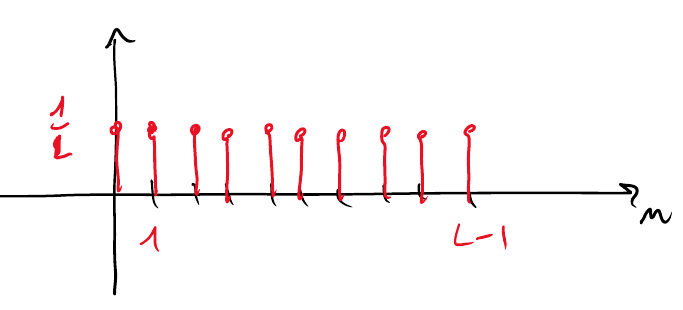
\includegraphics[scale=0.35]{immagini/lez15/es4RispostaImpulso.jpg}
\end{figure}

Il sistema che ha prodotto questa risposta all'impulso sara':

\[
    y[n] = \frac{1}{L} \sum_{k = 0}^{L-1} x[n-k]
\]

Calcolandone la risposta in frequenza:

\[
    H(e^{j \hat{\omega}}) = \sum_{k = 0}^{L-1} \frac{1}{L} e^{-j \hat{\omega} n} = \frac{1}{L} \sum_{k = 0}^{L-1} e^{-j \hat{\omega} n}
\]

Notiamo che questa e' una serie nota $\sum_{k = 0}^{L-1} q^k = \frac{1 - q^L}{1 - q}$, se chiamo $e^{-j \hat{\omega}} = q$, ottengo:

\[
    H(e^{j \hat{\omega}}) = \frac{1}{L} \frac{1 - e^{-j \hat{\omega}L}}{1 - e^{-j \hat{\omega}}}
\]

Ora come prima raccolgo la meta' dell'esponente massimo:

\[\begin{split}
    H(e^{j \hat{\omega}}) =& \frac{1}{L} \frac{e^{-j \hat{\omega} \frac{L}{2}}}{e^{-j \hat{\omega} \frac{L}{2}}} \frac{(e^{j \hat{\omega} \frac{L}{2}} - e^{-j \hat{\omega} \frac{L}{2}})}{(e^{j   \frac{\hat{\omega}}{2}} - e^{-j \frac{\hat{\omega}}{2}})} \frac{\textcolor{red}{2j}}{\textcolor{red}{2j}} \\
    =& e^{-j \hat{\omega} \frac{(L-1)}{2}} \frac{\sin(\hat{\omega} \frac{L}{2})}{\sin(\frac{\hat{\omega}}{2})} \cdot \frac{1}{L}
\end{split}\]

Ottenendo la forma di Dirichlet.

\section{Sistemi in cascata}
Quello che vogliamo fare e' prendere l'output di un sistema e metterlo in input ad un altro sistema LTI.

\begin{figure}[ht!]
    \centering
    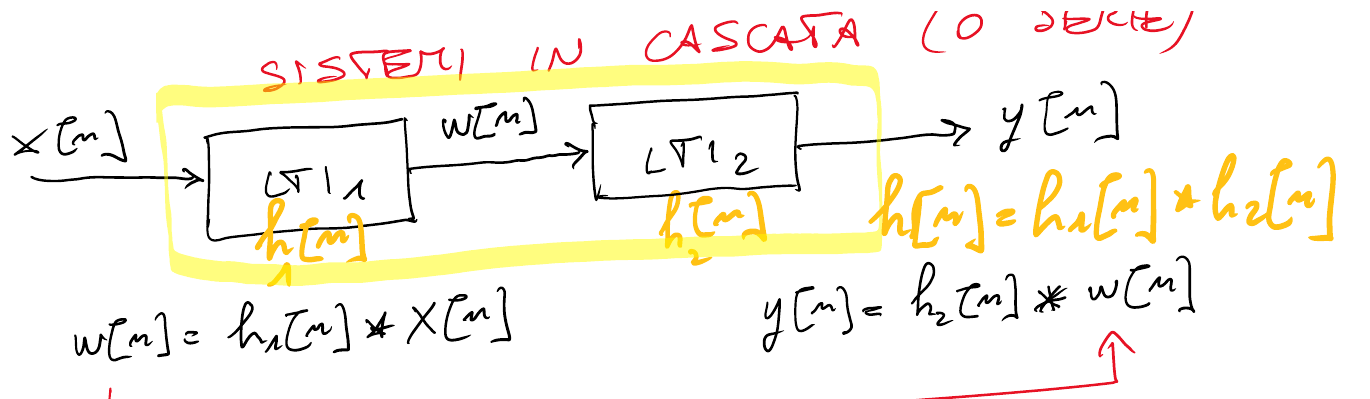
\includegraphics[scale=0.35]{immagini/lez15/sistemiCascata.jpg}
\end{figure}

\[\begin{split}
    y[n] &= h_2[n] * (h_1[n] * x[n]) \\
    y[n] &= (h_1[n] * h_2[n]) * x[n] \\
    h[n] &= h_1[n] * h_2[n]
\end{split}\]

\section{Parallelo di due sistemi}

\begin{figure}[ht!]
    \centering
    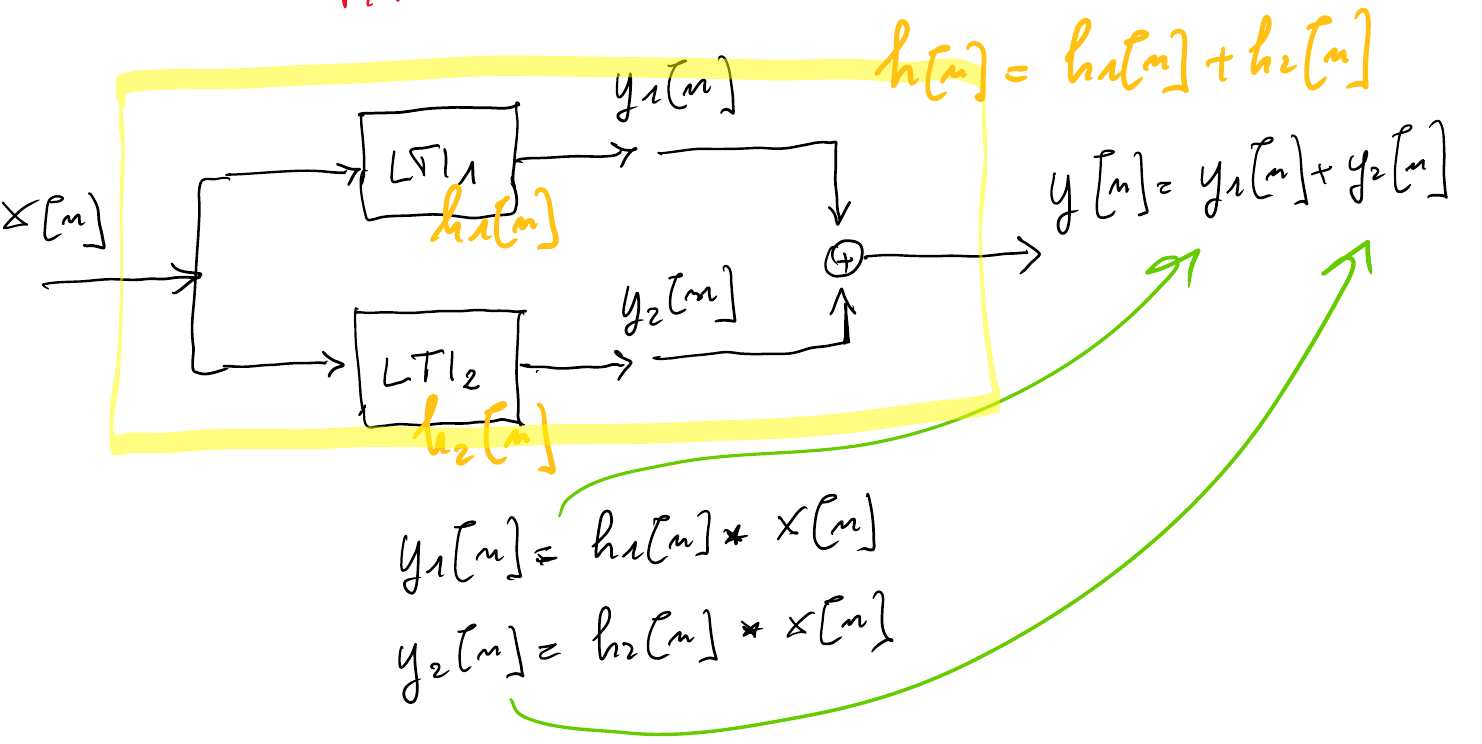
\includegraphics[scale=0.35]{immagini/lez15/paralleloSistemi.jpg}
\end{figure}

\[\begin{split}
    y[n] &= h_1[n] * x[n] + h_2[n] * x[n]\\
    y[n] &= (h_1[n] + h_2[n]) * x[n] \\
    h[n] &= h_1[n] + h_2[n]
\end{split}\]

